% Статья "Точная вероятность нарушения SLA в системах пакетного обслуживания
% с ограниченным размером пакета и фазовым временем обслуживания".
%
% Личный материал (не часть пакета most-queue, docs/статьи/ в .gitignore).
% Стиль оформления -- по образцу реальной опубликованной статьи автора в
% журнале "Труды Военно-космической академии имени А.Ф. Можайского".
%
% Сборка: latexmk -xelatex main.tex   (требуется XeLaTeX + biber)
%
% encoding: UTF-8
\documentclass[12pt,a4paper]{article}

\usepackage{geometry}
\geometry{top=2.5cm,bottom=2.5cm,left=3cm,right=2cm}

\usepackage{fontspec}
\setmainfont{PT Serif}
\newfontfamily\cyrillicfonttt{DejaVu Sans Mono}

\usepackage{polyglossia}
\setmainlanguage{russian}
\setotherlanguage[variant=american]{english}

\usepackage{amsmath,amssymb}
\usepackage{graphicx}
\usepackage{siunitx}
\sisetup{output-decimal-marker = {,}, group-separator = {\,}, retain-unity-mantissa = false}

\usepackage{array}
\usepackage{caption}
\usepackage{capt-of}
\usepackage{seqsplit}
\usepackage{xcolor}
\usepackage{tikz}
\usetikzlibrary{arrows.meta, positioning, shapes.geometric}
\captionsetup[figure]{labelsep=period, justification=centering, font=small, position=bottom}
\captionsetup[table]{labelsep=period, font={small,bf}, justification=raggedright, position=top}

\usepackage{indentfirst}
\setlength{\parindent}{1.25cm}
\linespread{1.12}

\usepackage[backend=biber, style=gost-numeric, sorting=none]{biblatex}
\addbibresource{../../bibliography/library.bib}

% Заголовки разделов: без нумерации, жирным, без капслока -- по образцу
% реальной статьи автора в "Трудах ВКА" (не ГОСТовский численный рубрикатор).
\newcommand{\articlesection}[1]{\par\vspace{14pt}{\bfseries #1}\par\vspace{6pt}\nopagebreak}

\newcommand{\keywordslabel}{\textbf{Ключевые слова: }}

\begin{document}
\sloppy

\noindent УДК 519.872

\bigskip
\noindent Р.С.~Хабаров

\noindent{\small [степень, звание, место работы --- заполнить]}

\bigskip
\begin{center}
\begin{minipage}{0.9\linewidth}
\centering
{\large\bfseries ТОЧНАЯ ВЕРОЯТНОСТЬ НАРУШЕНИЯ SLA В СИСТЕМАХ ПАКЕТНОГО ОБСЛУЖИВАНИЯ С ПОРОГОВЫМ ЗАПУСКОМ ПАКЕТА: НЕТЕРПЕНИЕ ЗАЯВОК И НЕСКОЛЬКО КАНАЛОВ}
\end{minipage}
\end{center}

\bigskip
\noindent\small
Рассмотрена система пакетного (batch-service) обслуживания с пороговым запуском пакета --- канал начинает обслуживание, как только накопится от $a$ до $b$ заявок, --- и временем обслуживания, зависящим от размера пакета; модель динамического батчинга при инференсе нейронных сетей, включая большие языковые модели (LLM). Предложен точный (не приближённый) метод вычисления вероятности нарушения SLA $P(W>D)$ для непрерывного времени, произвольного порога $1\le a\le b$ и фазового ($E_k$/$H_2$) времени обслуживания, зависящего от размера пакета, --- через PASTA-разложение времени ожидания и действие матричной экспоненты на явно построенный подгенератор; при $a>1$ разложение дополняется конструкцией <<гонки>> между новыми приходами и завершением уже обслуживаемых пакетов. Метод распространён на два практически значимых расширения: марковское (экспоненциальное) нетерпение заявок, для которого получена точная вероятность отмены запроса до начала его пакета, и система из $n$ независимых каналов с общей очередью (пул GPU-реплик), для которой при батч-размер-независимом времени обслуживания время ожидания точно сводится к уже решённой одноканальной конструкции с масштабированной ставкой. Все результаты точно регрессируют к известным частным случаям и подтверждены независимым имитационным моделированием. Численно показано, что повышение порога $a$ при фиксированном $b$ способно увеличить среднее время ожидания почти вдвое; что игнорирование нетерпения заявок маскирует падение истинной вероятности выполнения SLA с 99,9\,\% до 63\,\% видимым <<улучшением>> условного на <<дождался>> времени ожидания (эффект отбора выживших); и что добавление одной GPU-реплики в перегруженный пул снижает вероятность нарушения дедлайна более чем на порядок.

\medskip
\noindent\keywordslabel теория массового обслуживания, пакетное обслуживание, обслуживание, зависящее от размера пакета, фазовые распределения, SLA, вероятность нарушения дедлайна, нетерпеливые заявки, многоканальные системы, инференс больших языковых моделей, динамический батчинг.
\normalsize

\bigskip
\begin{center}
\begin{minipage}{0.9\linewidth}
\centering
{\bfseries EXACT SLA-VIOLATION PROBABILITY FOR THRESHOLD BATCH-SERVICE QUEUES: CUSTOMER ABANDONMENT AND MULTIPLE SERVERS}
\end{minipage}
\end{center}

\begin{center}
\small R.S.~Khabarov
\end{center}

\begin{otherlanguage}{english}
\small
We consider a batch-service queue with a threshold batch-formation rule --- the server starts a batch as soon as between $a$ and $b$ customers have accumulated --- and batch-size-dependent service time, the natural model for dynamic-batching neural-network (including large language model, LLM) inference. We derive an exact deadline-violation probability $P(W>D)$ for continuous time, any threshold $1\le a\le b$, and phase-type ($E_k$/$H_2$) batch-size-dependent service time, via a PASTA decomposition of the waiting time and matrix-exponential action on an explicitly constructed sub-generator; for $a>1$ the decomposition is extended with a race construction between new arrivals and the completion of already-in-service batches. The method is further extended in two practically significant directions: Markovian (exponential) customer abandonment, for which we derive the exact probability that a request is cancelled before its own batch starts; and a pool of $n$ independent servers sharing one queue (a GPU-replica pool), for which, under batch-size-independent service, the waiting time reduces exactly to the already-solved single-server construction with a rescaled rate. All results regress exactly to known degenerate cases and are validated against independent discrete-event simulation. Numerically, raising the threshold $a$ at a fixed $b$ can nearly double the mean wait; ignoring abandonment masks a drop in the true SLA-success probability from 99.9\% to 63\% behind an apparently \emph{improving} served-conditional wait time (a survivorship-bias effect); and adding one GPU replica to an overloaded pool cuts the deadline-violation probability by more than an order of magnitude.

\medskip
\noindent\textit{Key words:} queueing theory, batch service, batch-size-dependent service, phase-type distributions, SLA, deadline-violation probability, customer abandonment, multiserver systems, large language model inference, dynamic batching.
\end{otherlanguage}
\normalsize

\renewcommand{\figurename}{Рисунок}
\renewcommand{\tablename}{Таблица}

\articlesection{Введение}

Ускорение инференса нейронных сетей на графических процессорах (GPU) существенно опирается на динамический батчинг --- объединение нескольких независимо поступивших запросов в один пакет (batch), обрабатываемый каналом одновременно. Такое объединение повышает пропускную способность и энергоэффективность канала, но ценой дополнительной задержки: запрос вынужден дожидаться, пока сформируется пакет и пока этот пакет будет обслужен \cite{inoue2021}. Применительно к инференсу больших языковых моделей (LLM) данная задержка прямо входит в метрику времени до первого токена (time-to-first-token, TTFT), для которой операторы всё чаще формулируют требования к качеству обслуживания (SLO) в терминах вероятности, а не среднего значения: $P(\mathrm{TTFT}>D)<\varepsilon$ для заданного малого $\varepsilon$ \cite{quartz2026,jitserve2026}.

Два структурных свойства реальных систем динамического батчинга отличают их от классической модели пакетного обслуживания Бейли \cite{bailey1954}. Во-первых, время обслуживания пакета зависит от его размера: обработка пакета из $b$ заявок занимает больше времени, чем пакета из одной заявки, но не пропорционально $b$ --- типичная эмпирическая зависимость близка к линейной с положительным свободным членом \cite{inoue2021}. Во-вторых, размер пакета ограничен сверху: память GPU ограничивает максимальный размер батча $b_{\max}$, и на практике $b_{\max}$ --- конечное, зачастую небольшое число, а не абстрактная бесконечность.

Прямой практический прецедент --- работа Inoue \cite{inoue2021}, формулирующая сервер инференса как batch-service очередь с зависящим от размера пакета временем обслуживания и выводящая аналитическую оценку сверху среднего времени ожидания $E[W]$ в замкнутой форме при двух упрощающих допущениях: неограниченный максимальный размер пакета (при освобождении канала в пакет забираются все ожидающие заявки) и детерминированное, линейно зависящее от размера время обслуживания пакета. Автор прямо указывает, что точный анализ труден даже для зависящего от размера пакета $M/M/1$, и что для случая конечного $b_{\max}$ известен лишь алгоритмический, не дающий замкнутой формулы подход на основе матрично-аналитических методов \cite{neuts1989}.

Начиная с работы \cite{banerjee2012} и продолжая обширной серией последующих работ \cite{pradhan2016,banerjee2015,gupta2018,pradhan2024}, детально проработано точное стационарное распределение длины очереди (и содержимого канала) для систем пакетного обслуживания с зависящим от размера пакета, в том числе фазовым, временем обслуживания при различных входных потоках. Эти работы дают точное распределение длины очереди в различные моменты времени, но не распределение времени ожидания конкретной помеченной заявки. Классический результат для времени ожидания в системе пакетного обслуживания с общим, но не зависящим от размера пакета временем обслуживания получен точно методом корней характеристического уравнения \cite{chaudhry2023}; та же группа авторов, расширяя метод на коррелированный входной поток, называет полученное распределение времени ожидания эвристическим приближением \cite{banik2025} --- то есть даже без зависимости от размера пакета точное решение для коррелированного входа остаётся открытым. Единственная найденная нами работа, дающая хвост времени ожидания при обслуживании, зависящем от размера пакета, --- \cite{claeys2013}, но это дискретное время и заявленное самими авторами приближение.

Третье структурное свойство реальных систем динамического батчинга --- порог запуска пакета: канал не обязан начинать обслуживание по приходе первой же заявки, а может ждать накопления минимум $a$ заявок, чтобы не формировать заведомо неэффективные (по памяти/пропускной способности GPU) микро-пакеты. Этот порог $1\le a\le b$ присутствует в классической постановке Бейли \cite{bailey1954}, но ни одна из цитированных выше работ по зависящему от размера пакета обслуживанию не даёт для него точного времени ожидания непрерывного времени --- обобщение, требующее отдельной конструкции (см. раздел <<Метод>>) и составляющее часть вклада настоящей работы.

Наконец, два дополнительных структурных свойства реальных промышленных систем инференса --- нетерпение заявок и несколько параллельных каналов --- рассматриваются здесь впервые именно в сочетании с зависящим от размера пакета обслуживанием. Нетерпеливые заявки (отмена запроса, не дождавшегося начала обслуживания) классически моделируются экспоненциальным <<временем терпения>> начиная с модели Erlang-A \cite{garnett2002}; для систем пакетного обслуживания нетерпение изучалось лишь в ограниченной постановке --- например, \cite{vijayalaxmi2020} даёт транзиентный анализ батч-обслуживания с уходом заявок из очереди, но не точное стационарное распределение времени ожидания для непрерывного времени и не зависящее от размера пакета обслуживание. Несколько параллельных каналов батч-обслуживания также изучались --- недавняя работа \cite{bruneel2026} даёт точный анализ двух параллельных очередей с геометрическим батч-обслуживанием, но в дискретном времени и без общей очереди (каждая из двух очередей обслуживается своим каналом независимо, без разделения нагрузки) и без зависимости времени обслуживания от размера пакета. Таким образом, ни пересечение <<точно>>$\times$<<непрерывное время>>$\times$<<зависящее от размера пакета обслуживание>>$\times$<<нетерпение>>, ни то же пересечение с <<несколько каналов с общей очередью>> вместо <<нетерпение>> не закрыты ни одной из найденных работ.

Дальнейшая структура статьи следующая. Сначала приводится постановка задачи. Далее описан метод: базовая конструкция для произвольного порога $1\le a\le b$ и два её расширения --- нетерпение заявок и несколько каналов. После этого представлены результаты проверки и численные эксперименты, включая сравнение с оценкой \cite{inoue2021} и с приближением по моментам.

\articlesection{Постановка задачи}

Рассматривается одноканальная система $M/PH^{[a,b]}/1$: пуассоновский входной поток интенсивности $\lambda$; канал начинает обслуживание пакета, как только накопится не менее $a$ ожидающих заявок, и забирает в пакет $\min(b,j)$ заявок, где $j$ --- число ожидающих в момент запуска ($1\le a\le b$ --- общий порог запуска; $a=1$ --- вырожденный случай без накопления, канал запускает пакет по приходе первой же заявки); время обслуживания пакета размера $i$ имеет фазовое распределение --- $E_k$ (Эрланга порядка $k$ в нотации Кендалла) с темпом фазы $\mathrm{rate}(i)$ либо $H_2(p_1(i),\,\mu_1(i),\,\mu_2(i))$ --- с произвольной зависимостью параметров от $i$, в частности эмпирически наблюдаемой линейной зависимостью среднего от размера пакета \cite{inoue2021}.

Базовая цель --- точное $P(W>D)$ для $D\ge 0$, где $W$ --- время ожидания в очереди случайно выбранной (по PASTA) заявки, при любом $1\le a\le b$ и любом фазовом распределении обслуживания пакета. Эта базовая конструкция затем расширяется в двух ортогональных направлениях, каждое --- со своей областью применимости, не покрывающей полное прямое произведение всех рассмотренных обобщений одновременно:

\begin{itemize}
\item[1)] \textbf{Нетерпение заявок.} Каждая из $j$ ожидающих заявок независимо покидает очередь с постоянной ставкой $\gamma$ (марковское/беспамятное терпение, конвенция модели Erlang-A \cite{garnett2002}), если её обслуживание не началось. Цель --- точная вероятность того, что помеченная заявка покинет очередь до начала своего пакета, и точное условное (на <<дождалась>>) распределение $W$. Расширение получено для $E_k$-обслуживания, включая вырожденный экспоненциальный случай $k=1$.
\item[2)] \textbf{Несколько каналов обслуживания.} $n\ge 1$ идентичных каналов обслуживают пакеты из одной общей очереди --- модель пула из нескольких GPU-реплик за общим маршрутизатором запросов. Цель --- то же точное $P(W>D)$ для этой топологии. Расширение получено для батч-размер-независимого (экспоненциального) времени обслуживания.
\end{itemize}

\articlesection{Метод}

\noindent\textbf{Базовая конструкция, общий порог $1\le a\le b$.} Система моделируется усечённой по длине очереди ($j\le N$) цепью Маркова с состояниями $(i,\varphi,j)$, где $i\in\{0,\dots,b\}$ --- размер обслуживаемого пакета ($i=0$ --- простой), $\varphi$ --- текущая фаза обслуживания пакета (для $E_k$ --- номер пройденной фазы $0,\dots,k-1$, для $H_2$ --- выбранная при старте ветвь $\{0,1\}$), $j$ --- число ожидающих заявок. При $i=0$ (простой) канал накапливает заявки, не запуская пакет, пока $j<a$; по достижении $j=a$ немедленно запускается пакет размера ровно $a$ (заявки приходят по одной, переполнить порог одной заявкой невозможно). Стационарное распределение $\pi(i,\varphi,j)$ находится прямым решением $\pi Q=0$ для разреженного генератора $Q$.

На рисунке~\ref{fig:ctmc-diagram} приведена диаграмма переходов на примере $a=2$, $b=4$, $E_2$-обслуживания --- в том же духе, что диаграммы по ярусам для многофазных СМО \cite{ryzhikov2018}: состояния сгруппированы по ярусам числа ожидающих $j$ (снизу вверх), внутри яруса --- по микросостоянию $(i,\varphi)$ (слева направо). Горизонтальные стрелки --- переходы по фазе обслуживания пакета (не меняют $j$); вертикальные --- новые приходы (переход на ярус выше, $i,\varphi$ без изменений); диагональная --- завершение пакета: если $j<a$ (как на нижнем ярусе), канал простаивает; если $j\ge a$, немедленно стартует новый пакет размера $\min(b,j)$, что может изменить и размер $i$, и ярус сразу на несколько позиций --- это и есть источник <<гонки>> при $a>1$, разобранной ниже.

\begin{center}
\resizebox{\linewidth}{!}{%
\begin{tikzpicture}[
  every node/.style={font=\footnotesize},
  state/.style={ellipse, draw=black, thick, minimum width=13mm, minimum height=7mm, inner sep=0pt, align=center},
  idle/.style={state, fill=blue!12},
  sz2/.style={state, fill=green!18},
  sz3/.style={state, fill=orange!22},
  sz4/.style={state, fill=red!16},
  arr/.style={-{Stealth[length=2.2mm]}, thick, blue!55!black},
  ph/.style={-{Stealth[length=2.2mm]}, thick, black},
  dep/.style={-{Stealth[length=2.2mm]}, thick, purple!65!black},
  lvl/.style={font=\normalsize\bfseries, text=black!70},
]

\node[lvl] at (-1.7,0) {$0$};
\node[lvl] at (-1.7,2.1) {$1$};
\node[idle] (i0) at (0,0) {просто́й};
\node[idle] (i1) at (0,2.1) {просто́й};

\node[lvl] at (2.5,0) {$0$};
\node[sz2] (b0a) at (4.0,0) {$(2,0)$};
\node[sz2] (b0b) at (6.0,0) {$(2,1)$};

\node[lvl] at (2.5,3.05) {$\vdots$};
\node at (5.0,3.05) {\Large$\vdots$};

\node[lvl] at (2.5,6.1) {$j$};
\node[sz2] (bja) at (4.0,6.1) {$(2,0)$};
\node[sz2] (bjb) at (6.0,6.1) {$(2,1)$};
\node[sz3] (bjc) at (8.3,6.1) {$(3,0)$};
\node[sz3] (bjd) at (10.3,6.1) {$(3,1)$};
\node[sz4] (bje) at (12.6,6.1) {$(4,0)$};
\node[sz4] (bjf) at (14.6,6.1) {$(4,1)$};

\node[sz3, dashed] (res) at (14.6,9.3) {$(3,0)$};

\draw[arr] (i0) -- node[left]{$\lambda$} (i1);
\draw[arr] (i1) .. controls (1.0,3.8) and (2.6,2.2) .. node[above,pos=0.45,sloped]{$\lambda$: пакет $i{=}a$} (b0a);

\draw[ph] (b0a) -- node[above]{$\mu_2$} (b0b);
\draw[ph] (bja) -- node[above]{$\mu_2$} (bjb);
\draw[ph] (bjc) -- node[above]{$\mu_3$} (bjd);
\draw[ph] (bje) -- node[above]{$\mu_4$} (bjf);

\draw[dep] (b0b) .. controls (4.6,-2.6) and (0.6,-2.6) .. node[below,pos=0.5]{$\mu_2$: $j{<}a\Rightarrow$ простой} (i0);

\draw[arr] (b0a) -- node[right,pos=0.82]{$\lambda$} (bja);
\draw[arr] (b0b) -- node[right,pos=0.82]{$\lambda$} (bjb);

\draw[dep, dashed] (bjf) -- node[right, align=left]{$\mu_4$: $j\ge a\Rightarrow$\\[1pt] новый пакет $\min(b,j)$} (res);

\node[align=left, anchor=north west, font=\scriptsize] at (8.3,2.6) {
  \textcolor{blue!12!black}{\rule{2mm}{2mm}} простой ($i{=}0$)\\[1pt]
  \textcolor{green!35!black}{\rule{2mm}{2mm}} пакет $i{=}2$\\[1pt]
  \textcolor{orange!70!black}{\rule{2mm}{2mm}} пакет $i{=}3$\\[1pt]
  \textcolor{red!55!black}{\rule{2mm}{2mm}} пакет $i{=}4$\\[3pt]
  узел --- ключ $(i,\varphi)$; $\mu_i\equiv\mathrm{rate}(i)$
};
\end{tikzpicture}}
\captionof{figure}{Диаграмма переходов $(i,\varphi,j)$ на примере $a=2$, $b=4$, $E_2$-обслуживания; числа слева --- ярус $j$ (число ожидающих); верхний ярус --- произвольный $j\ge b$, нижний --- $j=0$ сразу после запуска первого пакета}
\label{fig:ctmc-diagram}
\end{center}

По свойству PASTA заявка, приходящая в систему, видит стационарное распределение $\pi(i,\varphi,j)$. Если канал простаивает ($i=0$) и $j=a-1$ (застигнутая заявка сама запускает пакет), $W=0$. Если канал простаивает и $j<a-1$, время ожидания сводится к ожиданию накопления недостающих заявок по пуассоновскому потоку: $\mathrm{Erlang}(a-j-1,\lambda)$ (при $a=1$ эта ветвь невозможна, что в точности сводит конструкцию к разобранному ранее случаю без порога).

Если канал занят, время ожидания раскладывается на остаток текущего обслуживаемого пакета ($E_{k-p}$ с темпом $\mathrm{rate}(i)$ для случая $E_k$, где $p$ --- застанная фаза; $\mathrm{Exp}(\mu_\varphi(i))$ для $H_2$ по марковости экспоненциальной фазы) и $\lfloor j/b\rfloor$ полных последующих пакетов размера~$b$ (каждый такой пакет впереди помеченной заявки всегда размера ровно $b$ --- иначе он включал бы помеченную заявку, что противоречит тому, что он сформирован до неё). При $a=1$ этого достаточно: остаток после полных пакетов впереди ($j\bmod b$ заявок) неизбежно $\ge0=a-1$, то есть не меньше порога минус единица, и собственный пакет помеченной заявки запускается немедленно, как только освобождается место. При $a>1$ возможна ситуация, когда остаток плюс помеченная заявка всё ещё не достигает порога $a$: тогда время ожидания определяется гонкой между новыми приходами (ставка $\lambda$) и оставшейся последовательностью фаз обслуживания пакетов впереди, поскольку приходы, случившиеся до завершения этих фаз, тоже засчитываются в порог. Конструкция --- двумерная поглощающая цепь, пересекающая <<какая фаза обслуживания сейчас идёт>> с <<сколько из недостающих $a-(j\bmod b)-1$ приходов уже случилось>>: с каждой фазы ставка $\lambda$ продвигает счётчик приходов (если он ещё не исчерпан), ставка завершения фазы продвигает фазу; достижение последней фазы с уже исчерпанным счётчиком поглощает цепь немедленно, иначе --- переход в хвост ожидания накопления по пуассоновскому потоку.

Для каждого занятого состояния $(i,\varphi,j)$ с $\pi(i,\varphi,j)>0$ (и для каждого простаивающего состояния с $j<a-1$) строится явный конечный подгенератор $T_{i,\varphi,j}$ поглощающей цепи Маркова, представляющей соответствующее разложение (начальный вектор $\alpha=e_1$, поглощение --- момент начала обслуживания помеченной заявки). Условный хвост времени ожидания --- классическая формула фазового распределения:
\begin{equation}
P(W>t \mid i,\varphi,j) = \alpha\exp(T_{i,\varphi,j}\,t)\,\mathbf{1}.
\label{eq:conditional-tail}
\end{equation}
Итоговый, безусловный точный хвост:
\begin{equation}
P(W>t) = \sum_{(i,\varphi,j)} \pi(i,\varphi,j)\,\alpha\exp(T_{i,\varphi,j}\,t)\,\mathbf{1}.
\label{eq:total-tail}
\end{equation}

Для $M/M/1$ и $M/E_k^{[a,b]}/1$ подгенератор $T$ --- последовательная (с хвостом накопления при $a>1$) матрица; для $H_2$ он содержит ветвление, а при $a>1$ ветвление пересекается со счётчиком приходов на последнем слое перед запуском пакета помеченной заявки (более ранние слои ветвятся независимо от счётчика). Экспонента вычисляется не явным построением плотной матрицы, а её действием на единичный вектор через разреженное представление.

При $b=1$ (отсутствие батчинга) результат должен точно совпасть с классической формулой хвоста $M/M/1$. При $k=1$ $E_k$-калькулятор должен точно совпасть с экспоненциальным (MM1) калькулятором; при $p_1=1$ $H_2$-калькулятор --- с тем же MM1-калькулятором. При $a=1$ (любой $b$) конструкция должна точно совпасть с разобранным ранее случаем без порога. Эти тождества --- не только регрессионные тесты, но и необходимое условие корректности построения.

\noindent\textbf{Расширение 1: нетерпение заявок.} Каждая из $j$ ожидающих заявок (независимо от того, занят канал или простаивает) покидает очередь со ставкой $\gamma$. Число заявок, стоящих впереди помеченной, при наличии нетерпения само становится процессом смерти (каждая из них может уйти независимо), идущим одновременно с формированием пакетов, а не фиксированной величиной, как в конструкции без нетерпения. Это требует явной размерности состояния $(R,K)$: $R$ --- число выживших впереди (убывает через нетерпение со ставкой $R\gamma$ и через полные пакеты впереди размера ровно $b$ --- то же структурное свойство, что и выше, по той же причине), $K$ --- новые приходы позади помеченной заявки (не влияют на исход формирования пакетов впереди, поскольку стоят в очереди после помеченной; достаточно отслеживать $K$ до порога $a-1$, после которого исход уже не зависит от точного значения $K$). Поглощение по двум конкурирующим типам --- <<обслужена>> (вектор ставок $r$, по одной на каждое состояние, где формируется пакет, включающий помеченную заявку) и <<ушла по терпению>> (общая ставка $\gamma$ из каждого состояния). Вероятность ухода и условные (на <<обслужена>>) моменты/хвост $W$ --- стандартные формулы фазового распределения с конкурирующим выходом:
\begin{equation}
P(\text{уход}) = \gamma\,\alpha\,(-T)^{-1}\mathbf{1}, \qquad
\mathrm{E}[W^n;\text{обслужена}] = n!\,\alpha\,(-T)^{-(n+1)}\,r,
\label{eq:abandonment}
\end{equation}
нормированные на $P(\text{обслужена})=1-P(\text{уход})$ для получения условных моментов. Расширение реализовано для $E_k$-обслуживания, включая вырожденный экспоненциальный случай $k=1$.

\noindent\textbf{Расширение 2: несколько каналов обслуживания.} $n$ идентичных каналов обслуживают пакеты из одной общей очереди. Состояние --- вектор занятости $(m_1,\dots,m_b)$ (число каналов, занятых пакетом размера $s$, $s=1,\dots,b$; $n-\sum m_s$ --- число свободных каналов), скрещенный с $j$. Пакет при хотя бы одном свободном канале запускается немедленно по достижении порога $a$ (той же конвенцией, что и при $n=1$) --- отсюда встроенный инвариант: свободный канал есть $\Rightarrow j<a$ (иначе он уже забрал бы заявки). Для батч-размер-независимого $\mu$ (ключевое упрощение, не предполагавшееся заранее) агрегированная ставка <<следующее освобождение>> среди всех $n$ занятых каналов равна ровно $n\mu$ независимо от состава занятости (по беспамятности экспоненциальных каналов и немедленному повторному запуску освободившегося канала), поэтому время ожидания помеченной заявки при всех занятых каналах не требует отслеживания вектора занятости вовсе: число заявок впереди убывает на $b$ при каждом событии-с-исключением со ставкой $n\mu$ --- в точности конструкция расширения~1 при $\gamma=0$ (без нетерпения) и единой ставкой $n\mu$ на всём протяжении (нет различия <<первый пакет vs последующие>>, поскольку нет понятия <<застигнутый пакет>>: любой из $n$ одинаковых каналов может освободиться следующим).

Все регрессионные тождества (по $b=1$, $k=1$, $p_1=1$ и, для базовой конструкции, по $a=1$; для расширений --- по $\gamma=0$ и по $n=1$) выполняются точно. Каждый результат, где регрессионные тождества неприменимы, независимо подтверждён имитационным моделированием, в том числе в точках глубокого хвоста, где точный результат даёт малое, но ненулевое значение.

\articlesection{Численные эксперименты}

\noindent\textbf{Эффект порога запуска $a$.} На параметрах \cite{inoue2021} ($\alpha=0{,}1438$, $\tau_0=1{,}8874$, $k=10$, $\lambda=0{,}8$), при фиксированном $b_{\max}=8$, повышение минимального порога запуска $a$ ощутимо ухудшает время ожидания, несмотря на неизменный максимальный размер пакета (таблица~\ref{tab:threshold-a}): накопление перед стартом пакета напрямую добавляет задержку, которую не компенсирует более редкий (и формально более <<эффективный>> по памяти GPU) запуск крупных пакетов. Операторы, повышающие $a$ ради экономии на формировании микро-пакетов при недогруженной системе, платят за это ощутимым ростом хвоста времени ожидания --- эффект, который ранее не из чего было точно оценить ($a=1$ был единственным разобранным случаем).

\begin{center}
\captionof{table}{Эффект порога запуска $a$ при фиксированном $b_{\max}=8$}
\label{tab:threshold-a}
\begin{tabular}{|c|c|c|c|}
\hline
$a$ & $\mathrm{E}[W]$ & $P(W>5)$ & $P(W>10)$ \\
\hline
1 & 1,074 & \num{2.74e-4} & \num{5.68e-9} \\
2 & 1,145 & \num{7.67e-3} & \num{1.36e-4} \\
4 & 1,978 & \num{8.51e-2} & \num{4.17e-3} \\
\hline
\end{tabular}
\end{center}

Для сравнения с оценкой \cite{inoue2021} использованы параметры эмпирической линейной подгонки автора для батч-инференса ResNet-50 на Tesla V100 ($\alpha=0{,}1438$, $\tau_0=1{,}8874$), $\lambda=0{,}8$ (устойчивая система при любом $b_{\max}\ge 2$: максимальная пропускная способность при $b_{\max}=2$ составляет $2/(2\alpha+\tau_0)\approx 0{,}92$). Аналитическая оценка \cite{inoue2021} в замкнутой форме для неограниченного батча: $\varphi(\lambda,\alpha,\tau_0)=3{,}353$.

\begin{center}
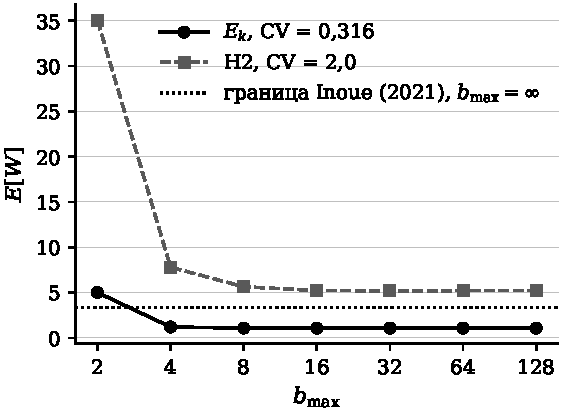
\includegraphics[width=0.62\linewidth]{../figures/fig1_mean_wait_vs_bmax.pdf}
\captionof{figure}{Истинное среднее время ожидания $E[W]$ в зависимости от $b_{\max}$ против границы \cite{inoue2021} ($\lambda=0{,}8$)}
\label{fig:mean-wait}
\end{center}

При малом (реалистичном для памяти GPU) $b_{\max}$ истинное среднее время ожидания превышает закрытую оценку \cite{inoue2021} --- несмотря на то, что последняя формально является оценкой сверху: граница корректно доказана для неограниченного батча и не распространяется на ограниченный случай. При коэффициенте вариации $CV=2$ (разумное предположение для пакета с запросами, смешанными по длине, типичными для LLM-инференса) расхождение при $b_{\max}=2$ достигает почти десятикратного значения. При больших $b_{\max}$, приближающихся к режиму \cite{inoue2021}, точное значение остаётся ниже границы --- граница верна именно там, где и была выведена, но не несёт информации о своей неприменимости при малом $b_{\max}$.

Поскольку параметры \cite{inoue2021} получены на ResNet-50-инференсе 2021~года, для независимой проверки того же качественного вывода на современном LLM-инференсе использованы измеренные данные Bench360 \cite{bench360_2026} (пропускная способность офлайн-пакетной обработки SGLang на GPU L4, таблица~4 источника): из зависимости токенов/с от размера батча $B\in\{16,32,64,128\}$ при фиксированной длине генерации восстановлена линейная аппроксимация $g(s)=\alpha s+\tau_0$ методом наименьших квадратов, $\alpha\approx0{,}076$~с, $\tau_0\approx6{,}30$~с --- на порядок больший фиксированный накладной расход на партию, чем в \cite{inoue2021}, что ожидаемо для декодирующего цикла LLM по сравнению со свёрточной сетью. При $\lambda=0{,}25$ (80\% от пропускной способности при $b_{\max}=2$) точное $E[W]$ по-прежнему превышает соответствующую границу \cite{inoue2021} при малом $b_{\max}$ (10,24 против 9,72 при $b_{\max}=2$) и быстро сходится к $\approx3{,}11$ уже при $b_{\max}=8$ --- то же качественное поведение, что и на синтетических параметрах, на независимо измеренных данных другого поколения оборудования и другого класса рабочей нагрузки.

\begin{center}
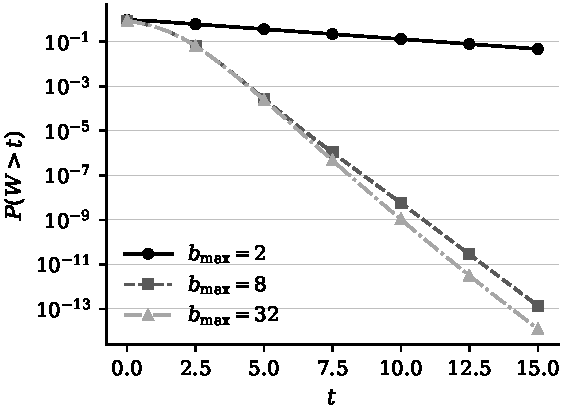
\includegraphics[width=0.62\linewidth]{../figures/fig2_exact_tail_curves.pdf}
\captionof{figure}{Точный хвост $P(W>t)$ для нескольких $b_{\max}$ ($E_k$, $CV=0{,}316$)}
\label{fig:tail-curves}
\end{center}

На рисунке~\ref{fig:tail-curves} видно, что форма хвоста существенно зависит от $b_{\max}$: при $b_{\max}=2$ (режим, близкий к границе устойчивости при выбранной нагрузке) хвост спадает заметно медленнее, чем при $b_{\max}=8$ и $b_{\max}=32$, кривые для которых практически совпадают --- система уже близка к своему пределу при неограниченном батче.

Для случая $E_k$ ($CV=0{,}316$) сравнивается точный хвост с результатом стандартного приёма <<подгонка 2--3 моментов под $H_2$ или гамма-распределение, вычисление хвоста подогнанного распределения>>, широко используемого на практике, когда точный метод недоступен.

\begin{center}
\captionof{table}{Точная и подогнанная по моментам вероятность $P(W>D)$}
\label{tab:exact-vs-fit}
\begin{tabular}{|c|c|c|c|c|}
\hline
$b_{\max}$ & $D$ & Точная $P(W>D)$ & Подогнанная (2 момента) & Отн. ошибка \\
\hline
2  & 5  & \num{3.7035e-1} & \num{3.7107e-1} & $+0{,}19\%$ \\
2  & 10 & \num{1.3255e-1} & \num{1.3331e-1} & $+0{,}57\%$ \\
2  & 20 & \num{1.6981e-2} & \num{1.6906e-2} & $-0{,}44\%$ \\
8  & 5  & \num{2.7386e-4} & \num{2.5296e-3} & $+824\%$ \\
8  & 10 & \num{5.6797e-9} & \num{2.4628e-6} & $+43\,261\%$ \\
8  & 20 & \num{3.3642e-18} & \num{1.6570e-12} & $+4{,}93\times10^{7}\%$ \\
16 & 5  & \num{2.4137e-4} & \num{2.5019e-3} & $+937\%$ \\
16 & 10 & \num{1.0582e-9} & \num{2.4014e-6} & $+226\,833\%$ \\
16 & 20 & \num{5.7739e-19} & \num{1.5685e-12} & $+2{,}72\times10^{8}\%$ \\
\hline
\end{tabular}
\end{center}

\bigskip
\noindent При умеренно глубоком хвосте ($b_{\max}=2$, где $D$ лишь в несколько раз превышает среднее) подгонка по двум моментам работает приемлемо (ошибка менее 1\%). Но при малом среднем времени ожидания и дедлайне, уходящем в действительно глубокий хвост --- во много раз больше среднего, типичный для GPU/LLM SLA-режима, где цель --- $P(\text{нарушение})<0{,}1\%$ --- подгонка по моментам систематически и резко переоценивает вероятность нарушения SLA: на один-два порядка при умеренной глубине хвоста и на много порядков при истинно глубоком хвосте.

\articlesection{Практические следствия: выбор $b_{\max}$ и предел приближений}

\noindent\textbf{Тождество баланса потоков.} Для любой стабильной эргодической системы пакетного обслуживания с $E[\text{длительность пакета}\mid\text{размер } s]=\alpha s+\tau_0$ (верно по построению и для $E_k$-, и для $H_2$-калькулятора, независимо от распределения длительности при фиксированном размере) коэффициент загрузки канала удовлетворяет точному тождеству
\begin{equation}
\rho = \lambda\alpha + \frac{\lambda\tau_0}{\bar S},
\label{eq:utilization}
\end{equation}
где $\bar S$ --- средний размер пакета, усреднённый по пакетам (не по заявкам). Тождество следует из теоремы о восстановлении с вознаграждением: интенсивность завершения пакетов в стационарном режиме $r=\lambda/\bar S$ (баланс потоков), а $\rho=r\cdot E[g(S)]=r(\alpha\bar S+\tau_0)$ по линейности $g$, без предположений о независимости размера пакета и его длительности.

Поскольку $\lambda\tau_0/\bar S$ убывает по $\bar S$, монотонность $E[W](b_{\max})$ (видимая на рисунке~\ref{fig:mean-wait}) сводится к монотонности $\bar S(b_{\max})$. Прямое траекторное доказательство этой монотонности наталкивается на реальное препятствие: система с большим $b_{\max}$ иногда формирует один большой и поэтому медленный пакет и временно отстаёт по числу завершённых заявок от системы с меньшим $b_{\max}$ --- полное доказательство остаётся открытой задачей. Тождество~\eqref{eq:utilization} тем не менее даёт проверяемый инструмент: обратное восстановление $\bar S=\lambda\tau_0/(\rho-\lambda\alpha)$ из уже посчитанной $\rho$ служит независимой сверкой корректности построения цепи Маркова и подтверждено точно на всех $b_{\max}$ обоих вариантов изменчивости (таблица~\ref{tab:utilization}).

\begin{center}
\captionof{table}{Коэффициент загрузки $\rho$ и восстановленный средний размер пакета $\bar S$}
\label{tab:utilization}
\begin{tabular}{|c|c|c|c|c|}
\hline
$b_{\max}$ & $\rho$ ($E_k$) & $\bar S$ ($E_k$) & $\rho$ ($H_2$) & $\bar S$ ($H_2$) \\
\hline
2  & 0,9580 & 1,79 & 0,9388 & 1,83 \\
4  & 0,8991 & 1,93 & 0,8172 & 2,15 \\
8  & 0,8948 & 1,94 & 0,7802 & 2,27 \\
16 & 0,8947 & 1,94 & 0,7688 & 2,31 \\
32 & 0,8947 & 1,94 & 0,7665 & 2,32 \\
\hline
\end{tabular}
\end{center}

\bigskip
\noindent\textbf{Минимальный $b_{\max}$ под целевой SLA.} Точный метод, применённый как чёрный ящик, даёт прямой прескриптивный результат: минимальный $b_{\max}$ --- наименьшее требование к памяти GPU на партию --- при котором $P(W>D)\le\varepsilon$ для заданного дедлайна $D$ и целевого уровня $\varepsilon$ (таблица~\ref{tab:minimal-bmax}, случай $E_k$). Для $H_2$ (высокая изменчивость) ни один из целевых уровней $\varepsilon\in\{10^{-2},10^{-3},10^{-4}\}$ не достижим ни при каком $b_{\max}\le128$ для $D\le30$ --- высокая изменчивость службы обслуживания фундаментально ограничивает то, чего можно добиться одним лишь укрупнением батчей; нужны либо более мягкий дедлайн, либо снижение изменчивости времени обслуживания другими средствами.

\begin{center}
\captionof{table}{Минимальный $b_{\max}$, при котором $P(W>D)\le\varepsilon$ (случай $E_k$)}
\label{tab:minimal-bmax}
\begin{tabular}{|c|c|c|c|}
\hline
$D$ & $\varepsilon=10^{-2}$ & $\varepsilon=10^{-3}$ & $\varepsilon=10^{-4}$ \\
\hline
5  & 4 & 8 & --- \\
10 & 4 & 4 & 4 \\
20 & 4 & 4 & 4 \\
30 & 2 & 4 & 4 \\
\hline
\end{tabular}
\end{center}

\bigskip
\noindent При существенно более глубоком дедлайне ($D=50$) данные вскрывают контринтуитивный, но воспроизводимый (устойчивый к удвоению усечения очереди $N$) эффект: точный хвост немонотонен по $b_{\max}$ --- $P(W>50)\approx7\times10^{-46}$ при $b_{\max}=8$--$16$, но вырастает до $\approx1,3\times10^{-39}$ при $b_{\max}=32$ (семь порядков хуже), хотя при умеренных дедлайнах больший $b_{\max}$ всегда не хуже. Причина --- та же, что ограничивает ценность асимптотики по $t\to\infty$: истинная скорость экспоненциального затухания хвоста равна $\mathrm{rate}(b_{\max})$ и убывает с ростом $b_{\max}$; при достаточно большом $D$ это в конце концов перевешивает выигрыш от более редких партий. На всех испытанных целевых уровнях $\varepsilon$ этот эффект не меняет практический ответ (провал остаётся на много порядков ниже любого разумного $\varepsilon$), но является строгим контрпримером к гипотезе о всеобщей монотонности.

\bigskip
\noindent\textbf{Предел однополюсных приближений.} Claeys et al. \cite{claeys2013} и предшествующая линия их работ оценивают хвост через доминирующую особенность (полюс, ближайший к началу координат) производящей функции задержки --- технику, по духу эквивалентную одной экспоненте, откалиброванной по истинной асимптотической скорости затухания. Точная формула их batch-size-зависимого расширения 2013~года нам недоступна (платный доступ), поэтому вместо попытки её повторить мы честно реализовали ту же общую технику для нашей модели: $P_{\text{approx}}(W>t)=\rho\exp(-\eta(b_{\max})\,t)$, где $\eta$ --- точная скорость затухания из раздела «Метод», а $\rho$ взято из таблицы~\ref{tab:utilization}. Результат (таблица~\ref{tab:dominant-pole}) --- систематическое и катастрофическое расхождение в обе стороны: при малом $b_{\max}$ однополюсное приближение на много порядков \emph{занижает} хвост (истинная асимптотика ещё не наступила, доминирует полиномиальная "выпуклость" тела распределения); при большом $b_{\max}$ оно на много порядков \emph{завышает} хвост (номинальная ставка $\mathrm{rate}(b_{\max})$ почти никогда не реализуется, поскольку большие партии при лёгкой загрузке формируются редко).

\begin{center}
\captionof{table}{Точный хвост против однополюсного приближения}
\label{tab:dominant-pole}
\begin{tabular}{|c|c|c|c|c|}
\hline
Режим & $b_{\max}$ & $D$ & Точная & Приближение \\
\hline
$E_k$ & 2   & 10 & \num{1.33e-1}  & \num{1.03e-20} \\
$E_k$ & 128 & 20 & \num{4.74e-19} & \num{4.69e-5}  \\
$H_2$    & 2   & 20 & \num{5.38e-1}  & \num{4.66e-2}  \\
$H_2$    & 128 & 20 & \num{3.90e-2}  & \num{5.55e-1}  \\
\hline
\end{tabular}
\end{center}

\articlesection{Расширение 1: нетерпеливые заявки}

На параметрах $a=2$, $b_{\max}=4$, $E_3$-обслуживание ($\alpha=0{,}1438$, $\tau_0=1{,}8874$), $\lambda=0{,}8$, таблица~\ref{tab:abandonment} показывает, как рост ставки терпения $\gamma$ влияет на три связанные, но различные величины: вероятность отмены запроса до начала его пакета $P(\text{уход})$, условное (на <<дождался>>) среднее время ожидания $\mathrm{E}[W\mid\text{обслужена}]$ и истинную вероятность выполнения SLA с дедлайном $D=10$ --- $P(\text{обслужена и }W\le D)$.

\begin{center}
\captionof{table}{Нетерпеливые заявки: вероятность ухода, условное время ожидания и истинный SLA-успех ($D=10$)}
\label{tab:abandonment}
\begin{tabular}{|c|c|c|c|}
\hline
$\gamma$ & $P(\text{уход})$ & $\mathrm{E}[W\mid\text{обслужена}]$ & $P(\text{обслужена и }W\le D)$ \\
\hline
0     & 0       & 1,541 & 0,9989 \\
0,02  & 0,0289 & 1,441 & 0,9706 \\
0,05  & 0,0666 & 1,328 & 0,9331 \\
0,10  & 0,1199 & 1,189 & 0,8800 \\
0,20  & 0,2042 & 0,994 & 0,7958 \\
0,50  & 0,3665 & 0,660 & 0,6335 \\
\hline
\end{tabular}
\end{center}

Третий и второй столбцы таблицы~\ref{tab:abandonment} движутся в противоположных направлениях, и в этом --- практически важная ловушка. Условное среднее время ожидания монотонно убывает с ростом $\gamma$ (с 1,541 до 0,660): это не улучшение системы, а классический эффект отбора выживших (survivorship bias) --- заявки, которым выпало бы долго ждать, с большей вероятностью уходят до того, как их дождавшееся собрат попадёт в выборку <<обслуженных>>, систематически смещая эту выборку в сторону коротких ожиданий. Если оператор системы измеряет только время ожидания уже обслуженных запросов (единственное, что обычно видно в логах эксплуатируемой системы --- отменённый запрос обычно не оставляет записи своего времени ожидания), метрика будет выглядеть всё лучше по мере роста нетерпения заявок, в то время как истинная вероятность успешного выполнения SLA (четвёртый столбец) рушится с 99,89\,\% до 63,35\,\%. Этот результат --- прямое практическое следствие точной конструкции раздела <<Метод>>: обе величины вычислены из одного и того же подгенератора, но отвечают на разные вопросы, и подмена одной другой --- систематическая, направленная ошибка, а не случайный шум измерения.

\articlesection{Расширение 2: несколько каналов обслуживания}

На тех же параметрах batch-size-зависимости среднего ($\alpha=0{,}1438$, $\tau_0=1{,}8874$), но с батч-размер-независимым экспоненциальным обслуживанием со средним, равным среднему при размере пакета 4 ($\mu=1/(4\alpha+\tau_0)\approx0{,}4061$ --- максимальная пропускная способность одного канала при $b_{\max}=4$ составляет $4\mu\approx1{,}624$), $a=2$, $b_{\max}=4$, общая интенсивность входного потока $\lambda=1{,}5$ (97,5\,\% от максимальной пропускной способности одного канала --- система с $n=1$ стабильна, но предельно нагружена), таблица~\ref{tab:multiserver} показывает эффект добавления идентичных каналов в общий пул с общей очередью.

\begin{center}
\captionof{table}{Эффект числа каналов $n$ при фиксированной суммарной нагрузке ($\lambda=1{,}5$)}
\label{tab:multiserver}
\begin{tabular}{|c|c|c|c|c|}
\hline
$n$ & $\mathrm{E}[W]$ & $P(W>5)$ & $P(W>10)$ & Загрузка канала \\
\hline
1 & 19,754 & 0,7633 & \num{5.97e-1} & 0,975 \\
2 & 1,144  & \num{2.95e-2} & \num{1.45e-3} & 0,739 \\
3 & 0,509  & \num{1.47e-3} & \num{5.63e-6} & 0,574 \\
4 & 0,370  & \num{3.15e-4} & \num{1.71e-7} & 0,454 \\
\hline
\end{tabular}
\end{center}

Переход от одного предельно нагруженного канала к двум ($n=1\to2$) снижает $\mathrm{E}[W]$ более чем в 17~раз и $P(W>5)$ --- более чем в 25~раз, хотя суммарная входная нагрузка не изменилась: с одним каналом система работает на грани устойчивости ($\rho=97{,}5\,\%$), и каждая дополнительная GPU-реплика пула не просто делит нагрузку поровну, а снимает именно ту часть перегрузки, которая отвечает за формирование длинного хвоста ожидания. При дальнейшем увеличении $n$ отдача убывает (переход $n=2\to3$ даёт более чем 20-кратное улучшение $P(W>5)$, а переход $n=3\to4$ --- <<лишь>> примерно 4,7-кратное) --- типичная для систем массового обслуживания картина убывающей отдачи от масштабирования числа каналов, здесь впервые точно, а не оценочно, количественно определённая для системы пакетного обслуживания с общей очередью. Практический вывод для оператора GPU-пула: при близкой к насыщению нагрузке одна дополнительная реплика значительно ценнее, чем может показаться по простому <<делению нагрузки на $n$>>.

\articlesection{Ограничения}

Базовая конструкция (общий порог $1\le a\le b$, фазовое обслуживание) ограничена одним каналом; расширения на нетерпение и на несколько каналов -- ортогональны и не объединены в единую конструкцию, покрывающую все обобщения одновременно. В частности: нетерпение реализовано для $E_k$-обслуживания (включая вырожденный экспоненциальный случай), но не для $H_2$ --- ветвящаяся структура $H_2$ требует пересечения ветвления каждого слоя впереди помеченной заявки с состоянием нетерпения, а не только последнего слоя (как для хвоста при $\gamma=0$), заметно более сложная конструкция, оставленная резервом. Несколько каналов реализовано для батч-размер-независимого (экспоненциального) обслуживания --- при батч-размер-зависимом обслуживании агрегированная ставка освобождения канала генуинно зависит от полного вектора занятости каналов, настоящий (не кажущийся) взрыв размерности состояния, тоже оставленный резервом. Нет конструкции, одновременно дающей, например, нетерпение и несколько каналов, или несколько каналов с фазовым (а не экспоненциальным) обслуживанием.

Основное численное сравнение использует параметры подгонки \cite{inoue2021} для ResNet-50-инференса; независимая проверка на измеренной пропускной способности современного LLM-инференса \cite{bench360_2026} переносит только среднюю зависимость $g(s)=\alpha s+\tau_0$, а не изменчивость времени обслуживания батча --- коэффициент вариации в обоих случаях остаётся синтетическим допущением, --- в целом это управляемое численное исследование, а не воспроизведение конкретной производственной системы. Сравнение с оценкой \cite{inoue2021} выполнено только по среднему; сравнение с подгонкой по моментам для хвоста выполнено только для случая $E_k$ низкой изменчивости. Монотонность $E[W](b_{\max})$ и $\bar S(b_{\max})$ подтверждена численно на всём испытанном диапазоне параметров, но не доказана в общем виде; как показано выше, при достаточно глубоком дедлайне сам точный хвост $P(W>D)$ немонотонен по $b_{\max}$ --- общее доказательство (или опровержение) монотонности остаётся открытой задачей. Численные примеры расширений (таблицы~\ref{tab:abandonment}--\ref{tab:multiserver}) --- иллюстративные, на одном наборе параметров каждый; систематическое исследование по сетке параметров (как для $b_{\max}$ в разделе <<Практические следствия>>) для этих двух расширений не проводилось.

\articlesection{Заключение}

Получена и верифицирована точная вероятность нарушения SLA для системы пакетного обслуживания с общим порогом запуска пакета $1\le a\le b$ и фазовым временем обслуживания произвольного коэффициента вариации, зависящим от размера пакета, --- результат, закрывающий пересечение условий, не покрытое ни классической линией работ по точному распределению длины очереди для обслуживания, зависящего от размера пакета, ни единственным известным приближённым, дискретно-временным результатом для хвоста времени ожидания с такой зависимостью. Метод распространён на марковское нетерпение заявок (точная вероятность отмены до начала обслуживания и условное время ожидания, для $E_k$-случая) и на пул из $n$ независимых каналов с общей очередью (точный результат для батч-размер-независимого обслуживания, сводящийся к одноканальной конструкции с масштабированной ставкой) --- ни одно из этих двух расширений в сочетании с batch-size-зависимым обслуживанием ранее точно не рассматривалось.

Численно показано, что пренебрежение ограничением размера пакета может занижать истинное среднее время ожидания почти на порядок, а приближение по моментам --- занижать точность оценки вероятности нарушения SLA в глубоком хвосте на несколько порядков; что повышение порога запуска $a$ при фиксированном $b_{\max}$ способно почти вдвое увеличить среднее время ожидания; что игнорирование нетерпения заявок маскирует падение истинной вероятности выполнения SLA с 99,9\,\% до 63\,\% за кажущимся улучшением условного времени ожидания (эффект отбора выживших); и что добавление одной GPU-реплики в предельно нагруженный пул снижает вероятность нарушения дедлайна более чем на порядок. Все эти эффекты напрямую релевантны практике SLA-ориентированного управления GPU/LLM-инференс-серверами. Дополнительно показано, что точный метод даёт прямой прескриптивный инструмент выбора минимального $b_{\max}$ под целевую SLA, и что альтернативная, однополюсная техника оценки хвоста (в духе Claeys et al. \cite{claeys2013}) расходится с точным значением на величину до $10^{14}$--$10^{19}$ в зависимости от режима. Открытая программная реализация всех описанных методов доступна в библиотеке most-queue \cite{mostqueue2026}.

\articlesection{Список литературы}
\printbibliography[heading=none]

\end{document}
